% !TEX TS-program = pdflatex
%===================================================================================================
% Beamer presentation: Explanation of the improved encoder-decoder translation notebook
%===================================================================================================
\documentclass[aspectratio=169]{beamer}

%===================================================================================================
% Theme and packages
%===================================================================================================
\usetheme{Madrid}
\usecolortheme{default}

\usepackage[utf8]{inputenc}
\usepackage[T1]{fontenc}
\usepackage{lmodern}
\usepackage{amsmath, amssymb}
\usepackage{booktabs}
\usepackage{array}
\usepackage{xcolor}
\usepackage{listings}
\usepackage{tikz}
\usetikzlibrary{arrows.meta, positioning, shapes.geometric}

%===================================================================================================
% Listings configuration
%===================================================================================================
\definecolor{codebg}{RGB}{248,248,248}
\definecolor{codegray}{RGB}{90,90,90}
\definecolor{codeblue}{RGB}{30,70,150}
\definecolor{codered}{RGB}{150,30,30}
\definecolor{codegreen}{RGB}{30,120,70}

\lstdefinestyle{pythonstyle}{
    language=Python,
    basicstyle=\ttfamily\scriptsize,
    keywordstyle=\color{codeblue}\bfseries,
    commentstyle=\color{codegreen},
    stringstyle=\color{codered},
    backgroundcolor=\color{codebg},
    numbers=left,
    numberstyle=\tiny\color{codegray},
    stepnumber=1,
    numbersep=5pt,
    showstringspaces=false,
    breaklines=true,
    frame=single,
    rulecolor=\color{black!25},
    tabsize=4,
    columns=fullflexible
}

\lstset{style=pythonstyle}

%
%===================================================================================================
%
\title[]{Chapter 3 Lab -- Encoder-Decoder Translation}
\subtitle{Advanced Machine Learning for Finance}
\author{Giovanni Della Lunga}
\institute{Master's Degree in Quantitative Finance -- University of Bologna}
\date{Bologna -- 2026}
%
%===================================================================================================
%

%===================================================================================================
\begin{document}
%===================================================================================================

%
%---------------------------------------------------------------------------------------------------
%
\begin{frame}
    \titlepage
\end{frame}
%__________________________________________________________________________
%
\begin{frame}[plain]
\centering
\vspace{1.0cm}
\LARGE{\textbf{Section 1}}
\vspace{0.5cm}

{\Huge \textbf{Lost in Translation}}

\vspace{1.5cm}

{\large
\begin{tabular}{@{}l l@{}}
\textbf{Notebooks:} 
& \texttt{06\_encoder-decoder\_translation\_with\_keras.ipynb} \\[0.3em]
& 
\end{tabular}
}

\end{frame}
%__________________________________________________________________________
%
\begin{frame}[fragile]{Motivation}
The notebook implements a small neural machine translation system.

\vspace{0.3cm}
Its goal is \textbf{educational}: it shows the basic mechanics of an LSTM-based encoder-decoder model before introducing more advanced architectures such as attention, and Transformers.

\end{frame}
%
%---------------------------------------------------------------------------------------------------
%
\begin{frame}[fragile]{Notebook workflow}
\begin{center}
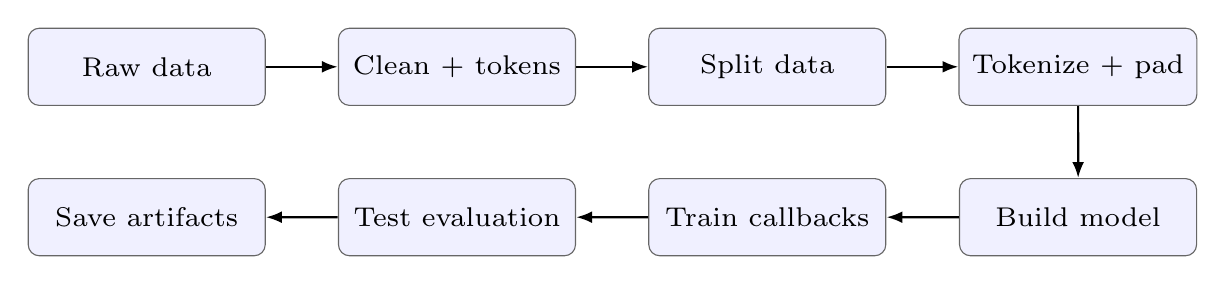
\begin{tikzpicture}[
    scale=1.4, transform shape,
    node distance=0.65cm,
    box/.style={rectangle, rounded corners, draw=black!60, fill=blue!6, minimum width=2.15cm, minimum height=0.70cm, align=center, font=\scriptsize},
    arrow/.style={-{Latex[length=2mm]}, thick}
]

\node[box] (raw) {Raw data};
\node[box, right=of raw] (clean) {Clean + tokens};
\node[box, right=of clean] (split) {Split data};
\node[box, right=of split] (tok) {Tokenize + pad};

\node[box, below=of raw] (save) {Save artifacts};
\node[box, below=of clean] (eval) {Test evaluation};
\node[box, below=of split] (train) {Train callbacks};
\node[box, below=of tok] (model) {Build model};

\draw[arrow] (raw) -- (clean);
\draw[arrow] (clean) -- (split);
\draw[arrow] (split) -- (tok);
\draw[arrow] (tok) -- (model);
\draw[arrow] (model) -- (train);
\draw[arrow] (train) -- (eval);
\draw[arrow] (eval) -- (save);

\end{tikzpicture}
\end{center}
\end{frame}
%
%---------------------------------------------------------------------------------------------------
%
\begin{frame}[fragile]{What problem are we solving?}
The model learns a mapping from a Spanish sentence to an English sentence.

\vspace{0.3cm}
Let
\[
    x = (x_1, x_2, \ldots, x_{T_s})
\]
be the Spanish input sequence, where:
\begin{itemize}
    \item $x_t$ is the token identifier at Spanish position $t$;
    \item $T_s$ is the maximum Spanish sequence length after padding.
\end{itemize}

Let
\[
    y = (y_1, y_2, \ldots, y_{T_e})
\]
be the English target sequence, where:
\begin{itemize}
    \item $y_t$ is the target English token identifier at output position $t$;
    \item $T_e$ is the maximum English sequence length after padding.
\end{itemize}
\end{frame}
%
%---------------------------------------------------------------------------------------------------
%
\begin{frame}[fragile]{Imports and reproducibility}
The notebook imports TensorFlow/Keras for neural networks, NumPy for arrays, and Pickle/JSON for saving artifacts.

\begin{lstlisting}
import os
import json
import pickle
import random
from pathlib import Path

import numpy as np
import tensorflow as tf

from tensorflow.keras.preprocessing.text import Tokenizer
from tensorflow.keras.utils import pad_sequences
from tensorflow.keras.models import Model, load_model
from tensorflow.keras.layers import Input, Embedding, Dense, LSTM
from tensorflow.keras.layers import RepeatVector, TimeDistributed, Activation
\end{lstlisting}
\end{frame}
%
%---------------------------------------------------------------------------------------------------
%
\begin{frame}[fragile]{Reproducibility settings}
The notebook fixes random seeds:

\begin{lstlisting}
RANDOM_SEED = 42
random.seed(RANDOM_SEED)
np.random.seed(RANDOM_SEED)
tf.random.set_seed(RANDOM_SEED)
\end{lstlisting}

\vspace{0.2cm}
This makes the experiment more reproducible, although perfect reproducibility may still depend on:
\begin{itemize}
    \item hardware;
    \item GPU kernels;
    \item TensorFlow version;
    \item low-level numerical libraries.
\end{itemize}
\end{frame}
%
%---------------------------------------------------------------------------------------------------
%
\begin{frame}[fragile]{Configuration block}
The notebook exposes the main choices in one place.

\begin{lstlisting}
START_ROW = 1000
END_ROW = 80000

VAL_SIZE = 0.10
TEST_SIZE = 0.10

BATCH_SIZE = 64
EPOCHS = 50
LEARNING_RATE = 1e-3

EMBEDDING_DIM = 128
LATENT_DIM = 64
DROPOUT_RATE = 0.20
\end{lstlisting}

This makes the experiment easier to modify.
\end{frame}
%
%---------------------------------------------------------------------------------------------------
%
\begin{frame}[fragile]{Data format}
The notebook expects a tab-separated bilingual file.

\vspace{0.3cm}
A typical row has the form:
\[
\texttt{English sentence} \quad \backslash t \quad \texttt{Spanish sentence}
\]

\vspace{0.3cm}
The code uses only the first two columns even if additional attribution columns are present.

\vspace{0.3cm}
This is a common structure for small translation datasets used in introductory sequence-to-sequence examples.
\end{frame}
%
%---------------------------------------------------------------------------------------------------
%
\begin{frame}[fragile]{Loading and parsing the file}
The notebook checks whether the file exists, reads all lines, and extracts valid English-Spanish pairs.

\begin{lstlisting}
with DATA_PATH.open("r", encoding="utf-8") as translation_file:
    raw_data = translation_file.read().splitlines()

raw_pairs = []
for row in raw_data:
    parts = row.split("\t")
    if len(parts) >= 2:
        english = parts[0].strip()
        spanish = parts[1].strip()
        if english and spanish:
            raw_pairs.append((english, spanish))
\end{lstlisting}

This produces a list of pairs such as:
\[
    (\text{English sentence}, \text{Spanish sentence}).
\]
\end{frame}
%
%---------------------------------------------------------------------------------------------------
%
\begin{frame}[fragile]{Text cleaning}
The cleaning function lowercases each sentence and removes punctuation.

\begin{lstlisting}
def clean_sentence(sentence: str) -> str:
    sentence = sentence.lower().strip()
    punctuation_to_remove = string.punctuation + "SPANISH_INVERTED_MARKS"
    sentence = sentence.translate(
        str.maketrans("", "", punctuation_to_remove)
    )
    sentence = " ".join(sentence.split())
    return sentence
\end{lstlisting}

\vspace{0.2cm}
This is deliberately simple. For a real translation system, punctuation should usually be handled more carefully because it carries syntactic information.
\end{frame}
%
%---------------------------------------------------------------------------------------------------
%
\begin{frame}[fragile]{Start and end tokens}
The notebook adds explicit boundary tokens to each English target sentence.

\begin{lstlisting}
START_TOKEN = "<start>"
END_TOKEN = "<end>"

english_target = f"{START_TOKEN} {english_clean} {END_TOKEN}"
\end{lstlisting}

\vspace{0.2cm}
These tokens teach the model that a target sentence has boundaries:
\begin{itemize}
    \item \texttt{<start>} marks the beginning of the target sequence;
    \item \texttt{<end>} marks the end of the target sequence.
\end{itemize}

They are especially important in more advanced decoders that generate one token at a time.
\end{frame}

%---------------------------------------------------------------------------------------------------
\begin{frame}[fragile]{Why train-validation-test split?}

\vspace{0.3cm}
The notebook uses:
\begin{itemize}
    \item \textbf{training set}: used to learn model weights;
    \item \textbf{validation set}: used during training to monitor generalization and stop early;
    \item \textbf{test set}: used only once for final evaluation.
\end{itemize}

\vspace{0.3cm}
The test set simulates genuinely unseen examples.
\end{frame}
%
%---------------------------------------------------------------------------------------------------
%
\begin{frame}[fragile]{Splitting indices}
The split is created by randomly permuting the example indices.

\begin{lstlisting}
def split_indices(n_samples, val_size, test_size, seed=42):
    rng = np.random.default_rng(seed)
    indices = rng.permutation(n_samples)

    n_test = int(round(n_samples * test_size))
    n_val = int(round(n_samples * val_size))

    test_idx = indices[:n_test]
    val_idx = indices[n_test:n_test + n_val]
    train_idx = indices[n_test + n_val:]

    return train_idx, val_idx, test_idx
\end{lstlisting}

The random seed makes the split reproducible.
\end{frame}
%
%---------------------------------------------------------------------------------------------------
%
\begin{frame}[fragile]{Tokenizer fitting without leakage}
The notebook fits tokenizers only on the training set.

\vspace{0.3cm}
This matters because validation and test data should remain unseen during model preparation.

\vspace{0.3cm}
If a tokenizer is fitted on the full dataset, then information from the validation and test sets leaks into preprocessing.

\vspace{0.3cm}
Unknown words in validation or test data are mapped to:
\[
    \texttt{<unk>}
\]
which stands for \textit{unknown token}.
\end{frame}
%
%---------------------------------------------------------------------------------------------------
%
\begin{frame}[fragile]{Creating Keras tokenizers}
The notebook creates one tokenizer for Spanish and one for English.

\begin{lstlisting}
def create_tokenizer(texts, oov_token=UNK_TOKEN):
    tokenizer = Tokenizer(oov_token=oov_token)
    tokenizer.fit_on_texts(texts)
    return tokenizer

spa_text_tokenizer = create_tokenizer(spa_train_text)
eng_text_tokenizer = create_tokenizer(eng_train_text)

spanish_vocab = len(spa_text_tokenizer.word_index) + 1
english_vocab = len(eng_text_tokenizer.word_index) + 1
\end{lstlisting}

The extra $+1$ accounts for the padding index $0$.
\end{frame}
%
%---------------------------------------------------------------------------------------------------
%
\begin{frame}[fragile]{Tokenization: from words to integers}
Tokenization converts a sentence into a sequence of integer identifiers.

\vspace{0.3cm}
For example:
\[
    \texttt{es una broma}
    \quad \longrightarrow \quad
    [12, 45, 381]
\]

\vspace{0.3cm}
The exact numbers depend on the tokenizer's learned vocabulary.

\vspace{0.3cm}
Neural networks do not process words directly; they process numerical tensors.
\end{frame}
%
%---------------------------------------------------------------------------------------------------
%
\begin{frame}[fragile]{Padding}
Sentences have different lengths, but neural networks process batches with fixed shapes.

\vspace{0.3cm}
Padding adds zeros after shorter sequences:
\[
    [12,45,381]
    \quad \longrightarrow \quad
    [12,45,381,0,0,0,0,0,0].
\]

\vspace{0.3cm}
The value $0$ is reserved for padding.

\vspace{0.3cm}
This is why padding-aware evaluation is necessary: padding is not a real word.
\end{frame}
%
%---------------------------------------------------------------------------------------------------
%
\begin{frame}[fragile]{Correct tensor shapes}
The notebook keeps Spanish inputs two-dimensional:

\begin{lstlisting}
X_train.shape == (n_train, max_spanish_len)
\end{lstlisting}

This is the correct input shape for a Keras \texttt{Embedding} layer.

\vspace{0.3cm}
The English targets are reshaped as:

\begin{lstlisting}
y_train.shape == (n_train, max_english_len, 1)
\end{lstlisting}

This is convenient for \texttt{sparse\_categorical\_crossentropy}, where each target position contains one integer class label.
\end{frame}
%
%---------------------------------------------------------------------------------------------------
%
\begin{frame}[fragile]{Model architecture}
\begin{center}

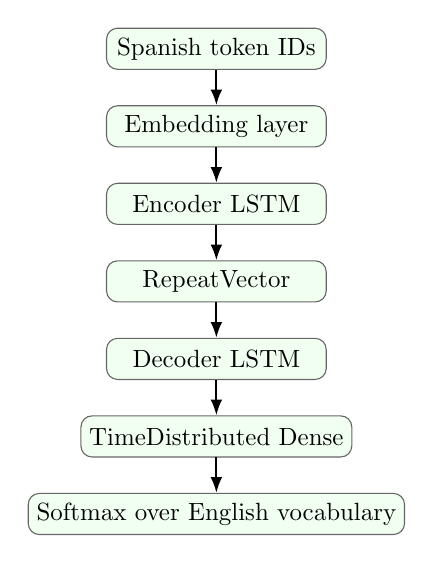
\begin{tikzpicture}[
    scale=0.90, transform shape,
    node distance=0.5cm,
    box/.style={rectangle, rounded corners, draw=black!60, fill=green!6, minimum width=3.1cm, minimum height=0.58cm, align=center},
    arrow/.style={-{Latex[length=2mm]}, thick}
]
\node[box] (input) {Spanish token IDs};
\node[box, below=of input] (emb) {Embedding layer};
\node[box, below=of emb] (enc) {Encoder LSTM};
\node[box, below=of enc] (rep) {RepeatVector};
\node[box, below=of rep] (dec) {Decoder LSTM};
\node[box, below=of dec] (dense) {TimeDistributed Dense};
\node[box, below=of dense] (soft) {Softmax over English vocabulary};

\draw[arrow] (input) -- (emb);
\draw[arrow] (emb) -- (enc);
\draw[arrow] (enc) -- (rep);
\draw[arrow] (rep) -- (dec);
\draw[arrow] (dec) -- (dense);
\draw[arrow] (dense) -- (soft);
\end{tikzpicture}

\end{center}
\end{frame}
%
%---------------------------------------------------------------------------------------------------
%
\begin{frame}[fragile]{Model construction}
The model is intentionally simple.

\begin{lstlisting}
input_sequence = Input(shape=(max_spanish_len,), name="spanish_input")

embedding = Embedding(
    input_dim=spanish_vocab,
    output_dim=EMBEDDING_DIM,
    mask_zero=True,
    name="spanish_embedding",
)(input_sequence)

encoder = LSTM(LATENT_DIM, return_sequences=False)(embedding)
r_vec = RepeatVector(max_english_len)(encoder)
decoder = LSTM(LATENT_DIM, return_sequences=True,
               dropout=DROPOUT_RATE)(r_vec)
logits = TimeDistributed(Dense(english_vocab))(decoder)
output = Activation("softmax")(logits)
\end{lstlisting}
\end{frame}
%
%---------------------------------------------------------------------------------------------------
%
\begin{frame}[fragile]{Embedding layer}
The embedding layer maps each Spanish token ID into a dense vector.

\vspace{0.3cm}
If the Spanish vocabulary size is $V_s$ and the embedding dimension is $d$, then the embedding matrix has shape:
\[
    V_s \times d.
\]

\vspace{0.3cm}
In the notebook:
\begin{itemize}
    \item $V_s$ is the Spanish vocabulary size;
    \item $d = 128$ is the embedding dimension.
\end{itemize}

The parameter \texttt{mask\_zero=True} tells the LSTM to ignore Spanish padding tokens.
\end{frame}
%
%---------------------------------------------------------------------------------------------------
%
\begin{frame}[fragile]{Encoder LSTM}
The encoder LSTM reads the whole Spanish sentence and compresses it into a single vector.

\vspace{0.3cm}
Mathematically, we can represent this as:
\[
    h = f_{\text{enc}}(x_1, x_2, \ldots, x_{T_s}),
\]
where:
\begin{itemize}
    \item $x_1, \ldots, x_{T_s}$ are Spanish token embeddings;
    \item $f_{\text{enc}}$ is the encoder LSTM transformation;
    \item $h$ is the final encoder vector.
\end{itemize}

\vspace{0.2cm}
In this notebook, $h$ has dimension $64$.
\end{frame}
%
%---------------------------------------------------------------------------------------------------
%
\begin{frame}[fragile]{The context-vector bottleneck}
The encoder-decoder architecture compresses the full source sentence into one vector.

\vspace{0.3cm}
This is useful pedagogically, because the architecture is easy to understand.

\vspace{0.3cm}
However, it also creates a bottleneck: all information needed for translation must pass through a single latent vector.

\vspace{0.3cm}
This is one reason why attention mechanisms became important in neural machine translation.
\end{frame}
%
%---------------------------------------------------------------------------------------------------
%
\begin{frame}[fragile]{RepeatVector}
The decoder must generate an English sequence of length $T_e$.

\vspace{0.3cm}
\texttt{RepeatVector} copies the encoder vector $h$ once for each target position:
\[
    h \quad \longrightarrow \quad (h, h, \ldots, h).
\]

\vspace{0.3cm}
This gives the decoder a sequence-shaped input.

\vspace{0.3cm}
The decoder then transforms these repeated context vectors into output hidden states.
\end{frame}
%
%---------------------------------------------------------------------------------------------------
%
\begin{frame}[fragile]{Decoder LSTM}
The decoder LSTM produces one hidden state for each English output position:
\[
    z_1, z_2, \ldots, z_{T_e}.
\]

Here:
\begin{itemize}
    \item $z_t$ is the decoder hidden state at English position $t$;
    \item $T_e$ is the padded English sequence length.
\end{itemize}

\vspace{0.3cm}
The notebook uses \texttt{return\_sequences=True} because we need an output prediction at every target time step.
\end{frame}
%
%---------------------------------------------------------------------------------------------------
%
\begin{frame}[fragile]{TimeDistributed Dense and Softmax}
At every output position, the model predicts a probability distribution over the English vocabulary.

\vspace{0.3cm}
For each decoder state $z_t$:
\[
    \hat{p}_t = \text{softmax}(W z_t + b),
\]
where:
\begin{itemize}
    \item $W$ is the output weight matrix;
    \item $b$ is the output bias vector;
    \item $\hat{p}_t$ is a probability vector over English tokens.
\end{itemize}

\vspace{0.2cm}
The predicted word is usually obtained with:
\[
    \arg\max_k \hat{p}_{t,k}.
\]
\end{frame}
%
%---------------------------------------------------------------------------------------------------
%
\begin{frame}[fragile]{Compilation}
The model is compiled with sparse categorical cross-entropy.

\begin{lstlisting}
enc_dec_model.compile(
    loss=sparse_categorical_crossentropy,
    optimizer=Adam(learning_rate=LEARNING_RATE),
    metrics=["accuracy", padding_aware_accuracy],
)
\end{lstlisting}

\vspace{0.2cm}
This loss is appropriate because each target word is represented as a single integer token ID, not as a one-hot vector.
\end{frame}
%
%---------------------------------------------------------------------------------------------------
%
\begin{frame}[fragile]{Loss function}
At each output position $t$, the model assigns a probability to every English token.

\vspace{0.3cm}
If the correct target token at position $t$ is $y_t$, and the predicted probability of that token is $\hat{p}_{t,y_t}$, then the cross-entropy contribution is:
\[
    -\log \hat{p}_{t,y_t}.
\]

\vspace{0.3cm}
The training loss averages this quantity over examples and target positions.
\end{frame}
%
%---------------------------------------------------------------------------------------------------
%
\begin{frame}[fragile]{Why standard accuracy can be misleading}
Standard token accuracy treats padding tokens as ordinary target tokens.

\vspace{0.3cm}
Example target:
\[
    [\texttt{<start>}, \texttt{its}, \texttt{a}, \texttt{joke}, \texttt{<end>}, 0, 0, 0]
\]

\vspace{0.3cm}
If the model learns to predict many zeros correctly, standard accuracy may become high even if real-word translation quality is mediocre.

\vspace{0.3cm}
Therefore, the notebook uses padding-aware accuracy.
\end{frame}
%
%---------------------------------------------------------------------------------------------------
%
\begin{frame}[fragile]{Padding-aware accuracy}
Padding-aware accuracy ignores target positions where the true token is $0$.

\vspace{0.3cm}
Let:
\begin{itemize}
    \item $y_{i,t}$ be the true token for example $i$ at position $t$;
    \item $\hat{y}_{i,t}$ be the predicted token;
    \item $m_{i,t}=1$ if $y_{i,t}\neq 0$, and $m_{i,t}=0$ otherwise.
\end{itemize}

Then:
\[
    \text{Accuracy}_{\text{masked}}
    =
    \frac{\sum_{i,t} m_{i,t} \mathbf{1}(y_{i,t}=\hat{y}_{i,t})}
         {\sum_{i,t} m_{i,t}}.
\]
\end{frame}
%
%---------------------------------------------------------------------------------------------------
%
\begin{frame}[fragile]{Padding-aware metric: implementation idea}
\begin{lstlisting}
def padding_aware_accuracy(y_true, y_pred):
    if len(y_true.shape) == 3:
        y_true = tf.squeeze(y_true, axis=-1)

    y_pred_ids = tf.argmax(y_pred, axis=-1, output_type=tf.int64)
    mask = tf.not_equal(y_true, 0)

    matches = tf.equal(y_true, y_pred_ids)
    matches = tf.logical_and(matches, mask)

    matches = tf.cast(matches, tf.float32)
    mask = tf.cast(mask, tf.float32)

    return tf.math.divide_no_nan(
        tf.reduce_sum(matches),
        tf.reduce_sum(mask)
    )
\end{lstlisting}
\end{frame}
%
%---------------------------------------------------------------------------------------------------
%
\begin{frame}[fragile]{Early stopping}
Early stopping monitors validation loss and stops training when it no longer improves.

\vspace{0.3cm}
This has two advantages:
\begin{itemize}
    \item it reduces unnecessary training time;
    \item it helps limit overfitting.
\end{itemize}

\vspace{0.3cm}
The notebook uses \texttt{restore\_best\_weights=True}, so the model is restored to the best validation-loss epoch.
\end{frame}
%
%---------------------------------------------------------------------------------------------------
%
\begin{frame}[fragile]{Checkpointing}
Checkpointing saves the best model observed during training.

\begin{lstlisting}
callbacks = [
    EarlyStopping(
        monitor="val_loss",
        patience=5,
        restore_best_weights=True,
        verbose=1,
    ),
    ModelCheckpoint(
        filepath=str(best_model_path),
        monitor="val_loss",
        save_best_only=True,
        verbose=1,
    ),
]
\end{lstlisting}

This is safer than using the final epoch by default.
\end{frame}
%
%---------------------------------------------------------------------------------------------------
%
\begin{frame}[fragile]{Training}
The model is trained on the training set, while validation data is used only for monitoring.

\begin{lstlisting}
history = enc_dec_model.fit(
    X_train,
    y_train,
    validation_data=(X_val, y_val),
    batch_size=BATCH_SIZE,
    epochs=EPOCHS,
    callbacks=callbacks,
)
\end{lstlisting}

\vspace{0.2cm}
The test set is not used during this phase.
\end{frame}
%
%---------------------------------------------------------------------------------------------------
%
\begin{frame}[fragile]{Training history}
The notebook plots:
\begin{itemize}
    \item training loss;
    \item validation loss;
    \item standard accuracy;
    \item padding-aware accuracy.
\end{itemize}

\vspace{0.3cm}
These plots help answer two important questions:
\begin{enumerate}
    \item Is the model learning on the training data?
    \item Is validation performance improving, or is the model overfitting?
\end{enumerate}
\end{frame}
%
%---------------------------------------------------------------------------------------------------
%
\begin{frame}[fragile]{Final evaluation on the test set}
The test set is used only after training is complete.

\vspace{0.3cm}
This gives a more honest estimate of how the model behaves on unseen data.

\vspace{0.3cm}
The notebook reloads the best checkpoint, then evaluates:
\begin{itemize}
    \item test loss;
    \item standard token accuracy;
    \item padding-aware token accuracy.
\end{itemize}
\end{frame}
%
%---------------------------------------------------------------------------------------------------
%
\begin{frame}[fragile]{Test evaluation code}
\begin{lstlisting}
if best_model_path.exists():
    enc_dec_model = load_model(
        best_model_path,
        custom_objects={
            "padding_aware_accuracy": padding_aware_accuracy
        },
    )

test_results = enc_dec_model.evaluate(
    X_test,
    y_test,
    batch_size=BATCH_SIZE,
    return_dict=True,
)
\end{lstlisting}

The custom metric must be provided when reloading the model.
\end{frame}
%
%---------------------------------------------------------------------------------------------------
%
\begin{frame}[fragile]{From probabilities to words}
The model does not directly output words.

\vspace{0.3cm}
At each English position, it outputs a probability vector over the vocabulary.

\vspace{0.3cm}
The decoding function applies:
\[
    \hat{y}_t = \arg\max_k \hat{p}_{t,k},
\]
where:
\begin{itemize}
    \item $\hat{p}_{t,k}$ is the probability of token $k$ at position $t$;
    \item $\hat{y}_t$ is the predicted token ID.
\end{itemize}
\end{frame}
%
%---------------------------------------------------------------------------------------------------
%
\begin{frame}[fragile]{Decoding utility}
\begin{lstlisting}
def logits_to_sentence(logits, tokenizer):
    index_to_word = build_index_to_word(tokenizer)
    predicted_token_ids = np.argmax(logits, axis=-1)
    return token_ids_to_sentence(
        predicted_token_ids,
        index_to_word
    )
\end{lstlisting}

\vspace{0.2cm}
The function also removes special tokens such as \texttt{<start>} and stops at \texttt{<end>}.
\end{frame}
%
%---------------------------------------------------------------------------------------------------
%
\begin{frame}[fragile]{Qualitative inspection}
Numerical metrics are not enough for translation.

\vspace{0.3cm}
The notebook therefore prints several examples from the held-out test set:
\begin{itemize}
    \item Spanish input;
    \item true English sentence;
    \item predicted English sentence.
\end{itemize}

\vspace{0.3cm}
This helps students see typical errors, not just aggregate performance numbers.
\end{frame}
%
%---------------------------------------------------------------------------------------------------
%
\begin{frame}[fragile]{Single-sentence inference}
The notebook includes a helper function for translating a new sentence.

\begin{lstlisting}
def translate_spanish_sentence(sentence, model=enc_dec_model):
    cleaned = clean_sentence(sentence)
    encoded = encode_and_pad(
        [cleaned],
        spa_text_tokenizer,
        max_spanish_len
    )
    prediction = model.predict(encoded, verbose=0)[0]
    return logits_to_sentence(prediction, eng_text_tokenizer)
\end{lstlisting}

This function applies the same preprocessing used during training.
\end{frame}
%
%---------------------------------------------------------------------------------------------------
%
\begin{frame}[fragile]{Saving artifacts}
A trained neural network is not enough by itself.

\vspace{0.3cm}
For future inference, we also need:
\begin{itemize}
    \item the Spanish tokenizer;
    \item the English tokenizer;
    \item maximum sequence lengths;
    \item special-token definitions;
    \item vocabulary sizes.
\end{itemize}

\vspace{0.3cm}
Without these objects, new input sentences cannot be encoded consistently with training.
\end{frame}
%
%---------------------------------------------------------------------------------------------------
%
\begin{frame}[fragile]{Saving model, tokenizers, and config}
\begin{lstlisting}
enc_dec_model.save(final_model_path)

with spanish_tokenizer_path.open("wb") as f:
    pickle.dump(spa_text_tokenizer, f)

with english_tokenizer_path.open("wb") as f:
    pickle.dump(eng_text_tokenizer, f)

config = {
    "max_spanish_len": max_spanish_len,
    "max_english_len": max_english_len,
    "spanish_vocab": spanish_vocab,
    "english_vocab": english_vocab,
}
\end{lstlisting}

The model and preprocessing pipeline must travel together.
\end{frame}
%
%---------------------------------------------------------------------------------------------------
%
\begin{frame}[fragile]{Reloading artifacts}
The final part of the notebook shows how to reload everything in a future session.

\vspace{0.3cm}
This is important because model deployment requires reproducible inference:
\begin{enumerate}
    \item load the saved model;
    \item load the tokenizers;
    \item load the configuration;
    \item apply the same cleaning, tokenization, and padding procedure.
\end{enumerate}
\end{frame}
%%===================================================================================================
%
\end{document}
%%===================================================================================================
%
